\documentclass[11pt]{article}
\usepackage[margin=.7in]{geometry}    
\usepackage[utf8]{inputenc}
\usepackage[english]{babel}

\usepackage{breakurl}
\usepackage{url}

\usepackage{adjustbox}
\usepackage{subcaption}
\captionsetup{
    font=small,
    labelfont=bf,
    margin=3em,
    compatibility=false
}

\usepackage{tabularx}
\usepackage{graphicx}
\usepackage{tikz}

\usetikzlibrary{automata,positioning,fit}

\title{Analysis of SMP Kernel Scheduling}

\author{Jnaneshwar Weibel}

% \affil{ 
% University of British Columbia, \authorcr
% Country             
% \authorcr \authorcr
% author1@xxx.xx
% \authorcr  \authorcr
% }

\begin{document}
\maketitle

\begin{abstract}
	As algorithms become larger and more resource intensive, computer hardware must become increasingly efficient to effectively run such programs.  In particular the capability for multiprocessing allows systems to distribute work across multiple CPUs.  Modern operating systems and their respective schedulers have the opportunity to make policy decisions, such as load balancing and locality of access to shared memory, when distributing programs that can influence the performance of both the kernel and user programs.
\end{abstract}

% \begin{keywords} 
% Word1, word2, word3.
% \end{keywords} 

% \tableofcontents

\section{Introduction}
\label{sec:introduction}
Hardware has evolved to become increasingly more complex and efficient, through areas such as processor frequency and memory latency.  Amdhal's law gives diminishing returns on the impact of parallelizing computation.  However, with respect to symmetric multiprocessing (SMP) in the kernel, Gustafon's law proves as now as a \textbf{scheduler?} can run ``in the same time with a larger workload'' \cite{gustafon}.  Thus as new system architectures take advantage of these processors.  They also require new approaches for system software and applications that run on top of this hardware \cite{nitrd}.

Within an operating system, the task scheduler is responsible for running user tasks and determining an execution order.  Yet with multiprocessing the scheduler offers an oporunity to distribute work across multiple cores.  In a preemptive system, the scheduler may migrate tasks between different cores which generally will incur a local penalty in cache performance yet may improve global performance.  Thus for this report several variations on the classical task scheduler will be compared to their impact on system performance and task scheduling.

A run-queue will consist of a FIFO list of tasks and will be protected by a run-queue specific lock.  The performance of several tasks will be measured using a single global run-queue, a per-core run-queue without pull migration, and a per-core run-queue with pull migration.  Pull migration refers to periodically re-balancing the load on two run-queues.  In addition, some tasks will be constrained to a smaller set of CPUs and thus may be fixed to a single process or not undergo push migration.  This paper will demonstrate the performance implications that various scheduling algorithms have on both local and global task execution.

\section{Environment?}
\label{sec:environment?}
The OS will be compiled for the ARMv8 (aarch64) instruction set and will be executed on the Raspberry Pi 3 B.  The device includes a 1.2 GHz 64-bit quad-core ARM Cortex-A53 processor and consists of a 16KB L1 data cache, a 16KB L1 instruction cache, and a 128KB L2 cache.  Intra-core cache coherency is enabled and uses the MOESI protocol \cite{arm-dcache-coherency}.  The memory address space is configured using a linear two level translation table with accessible memory configured as normal outer and inner write-back, write-allocate and device register memory configured as device nGnRnE.  Performance will be measured using the ARM Performance Monitor Unit (PMU) and the core timer.  The timer executes at a frequency of 19.2 MHz \cite{bcm2386} and each core maintains its own core timer which will preempt the current task each MS.  Both the kernel and pseudo-user processes will execute in EL1; however, the kernel will use SPx and the user processes will use SP0.

\section{Definitions?}
\label{sec:definitions?}

A ready queue can be defined as a generic data structure with two primary operations: ready and next.  For its internal manipulation a ready queue is protected by a spinlock.  Internally there are several queues corresponding to different priority levels allowing for processes with different priorities to be pushed onto the queues with no contention.  However, for discussion we will assume that all processes run at the same priority.

A naieve implementation for a SMP scheduler involves a global ready queue which all cores pull processes from.  This naieve implementation acts identical that in a single core system.  On SMP systems this data structure is benificial since it guarantees equal distribution of workload across all cores in addition to implementation simplicity.  Additionally, this workload distribution is not affected by a rapid stream of exiting processes.  However, the approach suffers from kernel lock contention since all cores must synchronize access to the queue.

\begin{figure*}[h!]
	\centering
	\begin{subfigure}{.48\linewidth}
		% \subfloat[Global Ready Queue]{
		% \centering
		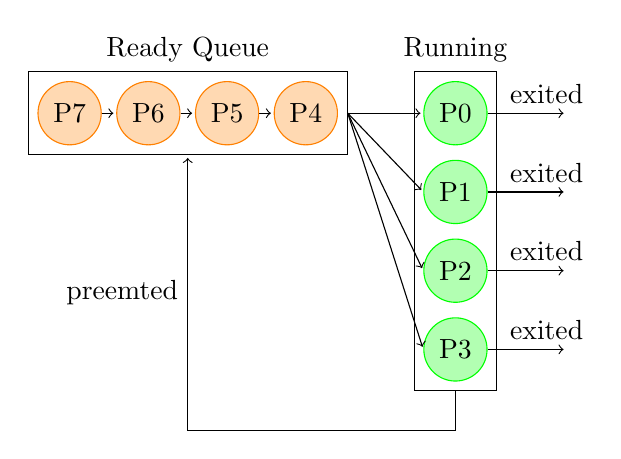
\begin{tikzpicture}[shorten >=1pt,node distance=1.0cm,on grid,auto,
				running/.style={circle, draw=green!100, fill=green!30},
				ready/.style={circle, draw=orange!100, fill=orange!30}
			]
			
			\node[ready] (p_4) [] {P4};
			\node[ready] (p_5) [left=of p_4] {P5};
			\node[ready] (p_6) [left=of p_5] {P6};
			\node[ready] (p_7) [left=of p_6] {P7};
			
			\node[state,rectangle] (q_0) [fit={(p_4) (p_5) (p_6) (p_7)}] [label=Ready Queue] {};
			
			\node[running] (r_0) [right=of q_0, xshift=24mm] {P0};
			\node[running] (r_1) [below=of r_0] {P1};
			\node[running] (r_2) [below=of r_1] {P2};
			\node[running] (r_3) [below=of r_2] {P3};
			
			\node[state,rectangle] (q_1) [fit={(r_0) (r_1) (r_2) (r_3)}] [label=Running] {};
			
			\draw[->] (q_0.east) -- (r_0.west);
			\draw[->] (q_0.east) -- (r_1.west);
			\draw[->] (q_0.east) -- (r_2.west);
			\draw[->] (q_0.east) -- (r_3.west);
			
			\draw[->] (p_7.east) -- (p_6.west);
			\draw[->] (p_6.east) -- (p_5.west);
			\draw[->] (p_5.east) -- (p_4.west);
			
			\draw[->] (r_0.east) -- ++(10mm,0) node[near end] {exited};
			\draw[->] (r_1.east) -- ++(10mm,0) node[near end] {exited};
			\draw[->] (r_2.east) -- ++(10mm,0) node[near end] {exited};
			\draw[->] (r_3.east) -- ++(10mm,0) node[near end] {exited};
			     
			\draw[->] (q_1.south) |- ++(0,-5mm) -| (q_0.south) node[near end] {preemted};
		\end{tikzpicture}
		\caption{Global Scheduling}
	\end{subfigure}
	% 
	\begin{subfigure}{.48\linewidth}
		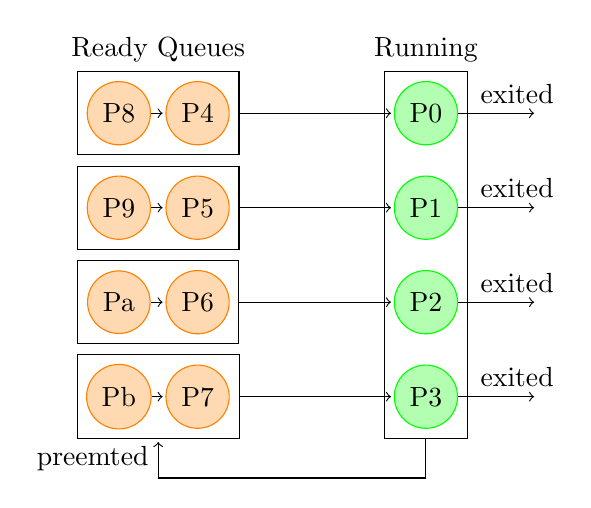
\begin{tikzpicture}[shorten >=1pt,node distance=1.0cm,on grid,auto,
				running/.style={circle, draw=green!100, fill=green!30},
				ready/.style={circle, draw=orange!100, fill=orange!30}
			]
			
			\node[ready] (p_4) [] {P4};
			\node[ready] (p_5) [below=of p_4, yshift=-2mm] {P5};
			\node[ready] (p_6) [below=of p_5, yshift=-2mm] {P6};
			\node[ready] (p_7) [below=of p_6, yshift=-2mm] {P7};
			
			\node[ready] (p_8) [left=of p_4] {P8};
			\node[ready] (p_9) [left=of p_5] {P9};
			\node[ready] (p_10) [left=of p_6] {Pa};
			\node[ready] (p_11) [left=of p_7] {Pb};    
			
			\node[state,rectangle] (q_0) [fit={(p_4) (p_8)}] [label=Ready Queues] {};
			\node[state,rectangle] (q_1) [fit={(p_5) (p_9)}] [below=of q_0, yshift=-2mm] {};
			\node[state,rectangle] (q_2) [fit={(p_6) (p_10)}] [below=of q_1, yshift=-2mm] {};
			\node[state,rectangle] (q_3) [fit={(p_7) (p_11)}] [below=of q_2, yshift=-2mm] {};
			
			\node[running] (r_0) [right=of q_0, xshift=24mm] {P0};
			\node[running] (r_1) [below=of r_0, yshift=-2mm] {P1};
			\node[running] (r_2) [below=of r_1, yshift=-2mm] {P2};
			\node[running] (r_3) [below=of r_2, yshift=-2mm] {P3};
			
			\node[state,rectangle] (q_r) [fit={(r_0) (r_1) (r_2) (r_3)}] [label=Running] {};
			
			\draw[->] (q_0.east) -- (r_0.west);
			\draw[->] (q_1.east) -- (r_1.west);
			\draw[->] (q_2.east) -- (r_2.west);
			\draw[->] (q_3.east) -- (r_3.west);
			
			\draw[->] (p_8.east) -- (p_4.west);
			\draw[->] (p_9.east) -- (p_5.west);
			\draw[->] (p_10.east) -- (p_6.west);
			\draw[->] (p_11.east) -- (p_7.west);
			     
			\draw[->] (q_r.south) |- ++(0,-5mm) -| (q_3.south) node[near end] {preemted};
			\draw[->] (r_0.east) -- ++(10mm,0) node[near end] {exited};
			\draw[->] (r_1.east) -- ++(10mm,0) node[near end] {exited};
			\draw[->] (r_2.east) -- ++(10mm,0) node[near end] {exited};
			\draw[->] (r_3.east) -- ++(10mm,0) node[near end] {exited};
		\end{tikzpicture}
		\caption{Per Core Ready Queue}
	\end{subfigure}
\end{figure*}

Under the current scheduler, a process, if eligible, is migrated during preemption.  In general the scheduler will opt to keep a process on the same CPU unless another core is sufficiently empty or its affinity set dictates otherwise.  In essence this rebalancing means that as processes are rescheduled, the cores will tend towards a balanced configuration.  However, it is also possible that a core will have a stream of processes terminate leading to a load imbalance between ready queues (fig. 3).

\begin{figure}[h]
	\centering
	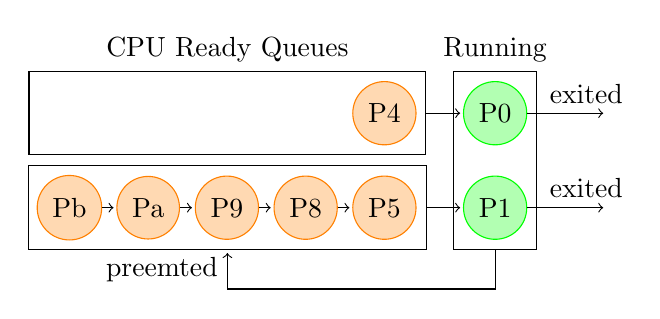
\begin{tikzpicture}[shorten >=1pt,node distance=1.0cm,on grid,auto,
			running/.style={circle, draw=green!100, fill=green!30},
			ready/.style={circle, draw=orange!100, fill=orange!30},
			empty/.style={circle, draw=none, fill=none, text=white}
		]
		
		\node[ready] (p_4) [] {P4};
		\node[ready] (p_5) [below=of p_4, yshift=-2mm] {P5};
		
		\node[ready] (p_6) [left=of p_5] {P8};
		\node[ready] (p_7) [left=of p_6] {P9};
		\node[ready] (p_8) [left=of p_7] {Pa};
		\node[ready] (p_9) [left=of p_8] {Pb}; 
		    
		\node[empty] (p_e) [above=of p_9, yshift=+2mm] {Pe};
		
		\node[state,rectangle] (q_0) [fit={(p_4) (p_e)}] [label=CPU Ready Queues] {};
		\node[state,rectangle] (q_1) [fit={(p_5) (p_6) (p_7) (p_8) (p_9)}] [below=of q_0, yshift=-2mm] {};
		
		\node[running] (r_0) [right=of q_0, xshift=24mm] {P0};
		\node[running] (r_1) [below=of r_0, yshift=-2mm] {P1};
		
		\node[state,rectangle] (q_r) [fit={(r_0) (r_1)}] [label=Running] {};
		
		\draw[->] (q_0.east) -- (r_0.west);
		\draw[->] (q_1.east) -- (r_1.west);
		
		\draw[->] (p_9.east) -- (p_8.west);
		\draw[->] (p_8.east) -- (p_7.west);
		\draw[->] (p_7.east) -- (p_6.west);
		\draw[->] (p_6.east) -- (p_5.west);
		     
		\draw[->] (q_r.south) |- ++(0,-5mm) -| (q_1.south) node[near end] {preemted};
		\draw[->] (r_0.east) -- ++(10mm,0) node[near end] {exited};
		\draw[->] (r_1.east) -- ++(10mm,0) node[near end] {exited};
	\end{tikzpicture}
	\caption{Unbalanced Scheduling}
\end{figure}

Pull migration is an effort to improve the rebalancing latency for queues which exhibit the behaivour in fig. 3.  Periodically, an idle core will search for an overloaded core and pull eligible processes from the tail of its queue.  This task requires locking the busy queue for a longer period of time; while, the idle queue tends to have have its lock acquired more frequently.  This task leads to high lock contention for both queues which can negatively impact the time spent in the kernel.  Specifically, while iterating, the busy core will be unable to retrieve the next runnable process.  Thus it is important to pick a large enough interval to do the rebalancing that it does not cause much strain on performance.  However, in most cases, if a core is not sufficiently loaded the pull migration task will instead exit prematurely instead of locking both cores.

\textbf{TODO: Process Fairness}


\section{Performance}
\label{sec:performance}
Different user programs were tested against the variations of the OS scheduler described previously.  In general the tests consist of performing a scalar multiply for a specified runtime.  These tests aim to simulate process cache access and utilization and provide repeatable results for user and kernel event counters.  For example, some examples heavily utilize memory while others operate on smaller subsets of data.  Additionally other processes are designed to run for longer or shorter periods of time to represent variability in task runtime.

While the actual measured runtime is presented in jiffies, these measurements should rarely be compared as they are rough measurements based on the CPU timer.  Additionally, tasks which may have a variable amount of IO with the FTDI output device are likely to see unrepresentative results compared to the actual execution of tasks.  Finally it is also important to note that all data fits into the L2 cache and thus pipeline stalls involved when fetching from main memory are limited the initial cold start.  \textbf{TODO: talk about the L2 cache in conclusion as it amplifies performance penalty}


\begin{figure*}[h]
	\centering
	% \makebox[\linewidth][c]{
	\begin{subtable}{.48\linewidth}
		\centering
		\begin{tabular}{ l|rrr }
			Type    & Total     & User      & Kernel  \\
			\hline
			Instrs  & 467617788 & 466380022 & 1237766 \\ 
			Cycles  & 693267321 & 691411106 & 1856215 \\ 
			Access  & 264291472 & 263665636 & 625836  \\ 
			Refill  & 1539      & 1340      & 199     \\ 
			Runtime & 45374884  & -         & -       \\ 
			\hline
		\end{tabular}
		\caption{single core - matrix 1x utilization}
	\end{subtable}
	\hfill
	\begin{subtable}{.48\linewidth}
		\centering
		\begin{tabular}{ l|rrr }
			Type    & Total      & User       & Kernel  \\
			\hline
			Instrs  & 1858506765 & 1853566311 & 4940454 \\ 
			Cycles  & 2768987855 & 2760678046 & 8309809 \\ 
			Access  & 1050488228 & 1047990323 & 2497905 \\ 
			Refill  & 1389770    & 1293188    & 96582   \\ 
			Runtime & 178608294  & -          & -       \\ 
			\hline
		\end{tabular}
		\caption{single core - matrix 4x utilization}
	\end{subtable}
\end{figure*}

This initial example aims to show the stark difference between process cache utilization.  Each example operates on a matrix fully utilizes the L1 cache and one which overloads the cache.  It is important to note that while the cycle count is nearly 4x larger as expected, the refill rate for the larger matrix is larger by a factor of nearly 900.  In these examples the most noticeable difference is the instructions per cycle in the kernel being roughly 11\% slower, due to the frequent thrashing of kernel memory. 

\textbf{TODO: note about how to improve global runtime in userspace programs}

\begin{figure*}[h]
	\centering
	% \makebox[\linewidth][c]{
	\begin{subtable}{.48\linewidth}
		\centering
		\begin{tabular}{ l|rrr }
			Type    & Total     & User      & Kernel  \\
			\hline
			Instrs  & 354249559 & 353629318 & 620241  \\ 
			Cycles  & 527538552 & 526403550 & 1135002 \\ 
			Access  & 200305644 & 199963039 & 342605  \\ 
			Refill  & 125708    & 116722    & 8986    \\ 
			Runtime & 41175374  & -         & -       \\ 
			\hline
		\end{tabular}
		\caption{multi core - global queue}
	\end{subtable}
	\begin{subtable}{.48\linewidth} 
		\centering        
		\begin{tabular}{ l|rrr }
			Type    & Total     & User      & Kernel \\
			\hline
			Instrs  & 375176881 & 374755150 & 421731 \\ 
			Cycles  & 556693572 & 556049701 & 643871 \\ 
			Access  & 212114934 & 211903384 & 211550 \\ 
			Refill  & 15332     & 14735     & 597    \\ 
			Runtime & 40603738  & -         & -      \\ 
			\hline
		\end{tabular}
		\caption{multi core - cpu queue (affinity)}    
	\end{subtable}
	% }
\end{figure*}

Extending the trivial example to multicore serves as a demonstration of easily parallelizable code and the benefit of process affinity.  When processor affinity is specified the number of kernel cycles is $76\%$ less than without which results in a $20\%$ improvement in instructions per cycle.  Again the improvement in kernel runtime is due to reduced thrashing of the kernel cores as evident in the lower APR.  However, there is also a $5\%$ loss in number of cycles, \textbf{TODO}.  Additionally it is important to note that the number of kernel instructions executed for the per core runqueue is $47\%$ less, owing to less scheduler lock contention between cores during a context switch.

\begin{figure*}[h]
	\centering
	% \makebox[\linewidth]{
	\begin{subtable}{.48\linewidth}
		\centering                 
		\begin{tabular}{l|rrr}
			Type    & Total      & User       & Kernel     \\
			\hline
			Instrs  & 1543135939 & 1396850683 & 146285256  \\ 
			Cycles  & 3146576481 & 2076522276 & 1070054205 \\ 
			Access  & 845516444  & 789349384  & 56167060   \\ 
			Refill  & 7653514    & 112360     & 7541154    \\ 
			Runtime & 152657484  & -          & -          \\
			\hline 
		\end{tabular}
		\caption{death - no pull (sm)}
	\end{subtable}
	\hfill
	\begin{subtable}{.48\linewidth}
		\begin{tabular}{l|rrr}
			Type    & Total      & User       & Kernel    \\
			\hline
			Instrs  & 1468299596 & 1398454567 & 69845029  \\ 
			Cycles  & 2552848279 & 2079318879 & 473529400 \\ 
			Access  & 816022596  & 790256656  & 25765940  \\ 
			Refill  & 3126952    & 140213     & 2986739   \\ 
			Runtime & 156804356  & -          & -         \\
			\hline
		\end{tabular}
		\caption{death - pulled (sm)}
	\end{subtable}
	% }
\end{figure*}

\begin{figure*}[h]
	% \makebox[\textwidth][c]{
	\begin{subtable}{.48\textwidth}
		\centering                 
		\begin{tabular}{l|rrr}       
			Type    & Total      & User       & Kernel     \\
			\hline
			Instrs  & 1613944771 & 1404552990 & 209391781  \\ 
			Cycles  & 3491698429 & 2086636583 & 1405061846 \\ 
			Access  & 873214573  & 793699999  & 79514574   \\ 
			Refill  & 9792188    & 28820      & 9763368    \\ 
			Runtime & 152321428  & -          & -          \\ 
			\hline
		\end{tabular}
		\caption{death - no pull (md)}
	\end{subtable}
	\hfill
	\begin{subtable}{.48\textwidth}
		\centering                 
		\begin{tabular}{l|rrr}  
			Type    & Total      & User       & Kernel    \\
			\hline
			Instrs  & 1520575475 & 1445743126 & 74832349  \\ 
			Cycles  & 2574353547 & 2147872630 & 426480917 \\ 
			Access  & 843643737  & 816978128  & 26665609  \\ 
			Refill  & 2283806    & 34930      & 2248876   \\ 
			Runtime & 161631896  & -          & -         \\ 
			\hline
		\end{tabular}
		\caption{death - pulled (md)}        
	\end{subtable}
	% }
\end{figure*}

% % TODO: Mention how the refill rate is significantly lower, instead of processes jumping around when they die, processes are moved which generally have lower cache impact as they are at the tail of runqueues

% A common pattern for distributing workload is to create many short lived processes which can perform independent computation before returning to a longer lived process.

For these examples, the impact of pull migration is immediately evident in the reduced cycle count of 75-80\% and a maximum reduction to 25\% of the original l1 refill rate to the same tests running without push migration.  Despite the apparent cache benefit it is important to note that the cycles spent in userspace tend to remain around the same meaning that the more important improvement ends up in the kernel.  When investigated more, it is noticable that the kernel cycle count and number of instructions executed drops significantly with pull migration.  Since the change in the kernel refill rate more insignificant this decrease in kernel overhead seems to be highly related to decreased lock contention between the cores.

This contention is derived from the scenario of multiple busy queues attempting to rapidly push work onto an idle queue.  In these cases, the added lock contention will inhibit processes from being scheduled on all cores since they are all effectively being serialized by the idle queue runqueue lock.  With pull migration, instead of having many repeated requests to the idle cores runqueue, a busy core elects to offload a larger amount of work until the idle core is no longer considered idle.  This prevents other cores from offloading work unnecesarily leading to improved userspace cache behaivour for those cores as well as reduced lock contention and minimal serialization.  Additionally, pulling processes from the end of the runqueue; instead of migrating recently executed processes, provides the opportunity to exhibit temporal locality and less cache pollution from more processes being executed. 

\textbf{TODO: cleanup these paragraphs}

\begin{figure*}[h]
	\centering
	% \makebox[\linewidth][c]{
	\begin{subtable}[b]{.48\linewidth}
		\centering                 
		\begin{tabular}{ l|rrr }
			Type    & Total      & User       & Kernel    \\
			\hline
			Instrs  & 2945961318 & 2829092653 & 116868665 \\ 
			Cycles  & 4881259967 & 4206238780 & 675021187 \\ 
			Access  & 1642115209 & 1598721424 & 43393785  \\ 
			Refill  & 4570467    & 298213     & 4272254   \\ 
			Runtime & 175864992  & -          & -         \\
			\hline
		\end{tabular}
		\caption{runtime - no pull}    
	\end{subtable}
	\hfill
	\begin{subtable}[b]{.48\linewidth}
		\centering
		\begin{tabular}{ l|rrr }
			Type    & Total      & User       & Kernel    \\
			\hline
			Instrs  & 2727027846 & 2625810066 & 101217780 \\ 
			Cycles  & 4421745433 & 3903078399 & 518667034 \\ 
			Access  & 1520521397 & 1483845439 & 36675958  \\ 
			Refill  & 3226996    & 222090     & 3004906   \\ 
			Runtime & 171909144  & -          & -         \\
			\hline
		\end{tabular}
		\caption{runtime - pulled}
	\end{subtable}
	% }
\end{figure*}

This case is important at showing the benefits of pull migration in relation to long term scheduling.  Specifically, since processes which execute for longer periods of time will undergo more context switches which incurs performance and leads to more kernel thrashing.  This example allows work to be migrated sooner and hence the total runtime decreases as well as the number of context switches.  In addition, since processes are moved from busy to idle cores, the user process cache utilization is more likely to be equally distributed across the processors \textbf{TODO: this sentence a little misworded}.  \textbf{TODO: mention size of data}

\begin{figure*}[h]
	\centering
	% \makebox[\textwidth][c]{
	\begin{subtable}{.48\textwidth}
		\centering
		\begin{tabular}{ l|rrr }
			Type    & Total      & User       & Kernel    \\
			\hline
			Instrs  & 836416320  & 753346040  & 83070280  \\ 
			Cycles  & 1724034904 & 1123196400 & 600838504 \\ 
			Access  & 456170314  & 426134109  & 30036205  \\ 
			Refill  & 4027452    & 231590     & 3795862   \\ 
			Runtime & 165276806  & -          & -         \\
			\hline
		\end{tabular}
		\caption{pool - unpooled sm}
	\end{subtable}
	\hfill
	\begin{subtable}{.48\textwidth} 
		\centering
		\begin{tabular}{ l|rrr }
			Type    & Total      & User       & Kernel    \\
			\hline
			Instrs  & 811243405  & 741653152  & 69590253  \\ 
			Cycles  & 1789217832 & 1113471653 & 675746179 \\ 
			Access  & 444450115  & 419398612  & 25051503  \\ 
			Refill  & 4540858    & 379326     & 4161532   \\ 
			Runtime & 66534692   & -          & -         \\
			\hline
		\end{tabular}
		\caption{pool - pooled sm}        
	\end{subtable}
	% }
\end{figure*}

\begin{figure*}[h]
	\begin{subtable}{.48\textwidth} 
		\centering
		\begin{tabular}{ l|rrr }
			Type    & Total      & User       & Kernel    \\
			\hline
			Instrs  & 819345284  & 755845609  & 63499675  \\
			Cycles  & 1672284752 & 1125235476 & 547049276 \\
			Access  & 450878090  & 427546852  & 23331238  \\
			Refill  & 3740754    & 148469     & 3592285   \\
			Runtime & 167143162  & -          & -         \\
			\hline
		\end{tabular}
		\caption{pool - unpooled}
	\end{subtable}
	\hfill
	\begin{subtable}{.48\textwidth} 
		\centering
		\begin{tabular}{ l|rrr }
			Type    & Total      & User       & Kernel    \\
			\hline
			Instrs  & 840132648  & 753613514  & 86519134  \\
			Cycles  & 1849770029 & 1127098953 & 722671076 \\
			Access  & 457128942  & 426166739  & 30962203  \\
			Refill  & 4435166    & 143616     & 4291550   \\
			Runtime & 66158114   & -          & -         \\
			\hline
		\end{tabular}
		\caption{pool - pooled}
	\end{subtable}
\end{figure*}

\textbf{TODO: remeasure runtimes? repeat tests with different MD case?}
\textbf{TODO: mention that these were unexpected, was expecting much better performance with the pooled - md}
This example has ipc larger in both cases.    However, one noticeable factor is that for larger sample size there is less l1 thrashing relavent in the APR (contributing factor for larger runtimes).  Instead for the smaller case the caches are able to be fully utilized.

\section{Lessons Learned}
\label{sec:lessons}

\section{Conclusion}
\label{sec:conclusion}

Conclusions here \cite{freebsd} \cite{unix}.

\section{Future Work}
\label{sec:future}

% \section{Acknowledgements} 

\onecolumn
\begin{sloppypar}
	\bibliographystyle{acm}
	\bibliography{biblio}
\end{sloppypar}

% \end{multicols}
\end{document}